% !TEX program = lualatex
% ---------------------------------------------------------------------------
% Лекция «Оптимизация логистических сетей» (2 академических часа).
% Курс «Методы анализа сетевых структур», НИУ ВШЭ -- Нижний Новгород, 2027.
%
% Основа: доклад на «Импульсе» 2026 (репозиторий Optimal-Logistic-Net,
% presentations/impulse2026), конспект 2026/lectures/Optimal-Logistics-Network.md
% и конкурс 2026/optimal-logistic-network-contest.
% Рисунки и figs/demo_numbers.tex строит make_figs.py (см. README.md рядом).
% Сборка: make -C .. lecture  или  latexmk в этой папке с TEXINPUTS=../theme//:
% ---------------------------------------------------------------------------
\documentclass[aspectratio=169,10pt]{beamer}
\usetheme{HSEnet}
\usepackage[russian]{babel}
\usepackage{amsmath,amssymb,mathtools}
\usepackage{booktabs,array}
\usepackage{pgfplots}
\pgfplotsset{compat=1.18}
\usetikzlibrary{arrows.meta,positioning,calc,shapes.geometric,fit,backgrounds}
\usepackage{qrcode}

% Роли цветов в лекции (все -- из палитры брендбука)
\colorlet{cStep}{hsePurple}   % машины, ступенька стоимости
\colorlet{cCap}{hseRed}       % ёмкость склада
\colorlet{cN1}{hseLightBlue}  % окрестность N1
\colorlet{cN2}{hseOrange}     % окрестность N2
\colorlet{cN3}{hseRed}        % окрестность N3
\colorlet{cOK}{hseGreen}      % хорошее решение

\tikzset{
  storage/.style={circle,draw=hseBlue,thick,fill=hsePale,minimum size=7mm,inner sep=0pt,font=\small},
  road/.style={-{Latex[length=2mm]},draw=hseBlue!60,thick},
  flow/.style={-{Latex[length=2.5mm]},draw=hseOrange,line width=2pt},
  box/.style={draw=hseBlue,thick,rounded corners=2pt,fill=hseBg,align=center,font=\small,inner sep=5pt,minimum height=9mm},
  lbl/.style={font=\scriptsize,text=hseBlue},
  bbnode/.style={draw=hseBlue,thick,rounded corners=2pt,fill=white,align=center,font=\scriptsize,inner sep=3pt},
}

\newcommand{\Real}{\mathbb{R}}
\newcommand{\Int}{\mathbb{Z}}
\newcommand{\ovl}{\mathit{overload}}
\newcommand{\load}{\mathit{load}}
\newcommand{\gapLB}{gap_{\mathrm{LB}}}

\InputIfFileExists{figs/demo_numbers.tex}{}{}

\course{Методы анализа сетевых структур}
\title{Оптимизация логистических сетей}
\subtitle{Многопродуктовые потоки, целочисленное программирование и~поиск с~чередующимися окрестностями}
\author{Александр Пономаренко}
\institute{НИУ ВШЭ -- Нижний Новгород, магистратура «Интеллектуальный анализ данных»}
\date{2027}

\begin{document}
\maketitle

\begin{frame}{План лекции}
\begin{columns}[T]
\column{0.55\textwidth}
\begin{enumerate}\setlength{\itemsep}{5pt}
\item Логистическая сеть как граф: что оптимизируем и почему это трудно
\item Потоки в сетях: от одного товара к многопродуктовому потоку (MCF)
\item Целочисленное программирование: модель, линеаризация, ветви и границы
\item Большие задачи: генерация столбцов, лагранжева релаксация, эвристики
\item GVNS с MILP-решателем (матэвристика): окрестности на примере реальной сети
\item Результаты на открытом наборе из 50 сетей и практика
\end{enumerate}
\column{0.42\textwidth}
\begin{block}{Цели лекции}
\begin{itemize}
\item записать логистическую задачу в виде MILP
\item понять, почему MILP-решатели (солверы) не справляются с большими сетями
\item сочетать эвристику с точным решателем
\item корректно сравнивать алгоритмы при неизвестном оптимуме
\end{itemize}
\end{block}
\end{columns}
\end{frame}

% ===========================================================================
\section{Логистическая сеть как граф}

\begin{frame}{Где возникают сетевые потоки}
\begin{columns}[T]
\column{0.5\textwidth}
\begin{itemize}\setlength{\itemsep}{5pt}
\item \textbf{транспорт}: грузовики между сортировочными центрами, железнодорожные составы, чартерные рейсы
\item \textbf{цепочки поставок}: завод $\to$ склад $\to$ магазин
\item \textbf{энергетика}: перетоки по линиям электропередачи
\item \textbf{связь}: маршрутизация трафика в сетях передачи данных
\end{itemize}
\column{0.5\textwidth}
\begin{block}{Общая модель}
\begin{itemize}
\item вершины --- склады, заводы, распределительные центры, потребители
\item рёбра --- маршруты с пропускной способностью и стоимостью
\item заявки --- какой груз, откуда, куда и в каком объёме перевезти
\end{itemize}
\end{block}
\takeaway{Цель --- выполнить все заявки с минимальными затратами, не нарушив ограничений.}
\end{columns}
\end{frame}

\begin{frame}{Сеть сортировочных центров}
\begin{columns}[T]
\column{0.5\textwidth}
\centering
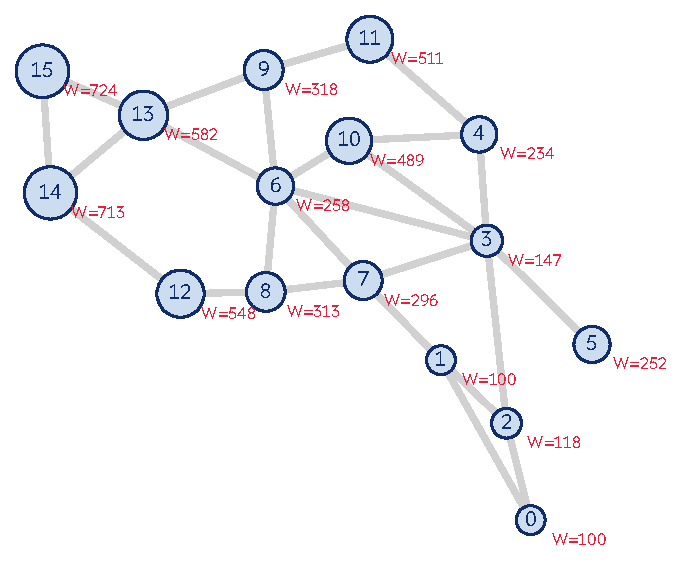
\includegraphics[height=0.66\textheight]{figs/belgium_roads.pdf}
\source{Бельгия из открытого набора: 16 складов, 180 заявок; размер узла --- ёмкость $W_v$}
\column{0.5\textwidth}
\begin{itemize}\setlength{\itemsep}{5pt}
\item \textbf{склады} $v\in V$: перегрузить можно не больше \textcolor{cCap}{$W_v$} единиц, единица перегруза стоит $f_v$
\item \textbf{дороги} $e\in E$: рейс машины стоит \textcolor{cStep}{$c_e$}, в машину входит $C=50$ единиц
\item \textbf{заявки} $k\in K$: перевезти $d_k$ единиц из $s_k$ в $t_k$; допускается перегрузка на промежуточных складах
\end{itemize}
\begin{block}{Что ищем}
маршруты и объёмы для всех заявок разом:\\[3pt]
\centerline{рейсы $+$ перегрузы $\to\min$}
\end{block}
\end{columns}
\end{frame}

\begin{frame}{Заявки на перевозку}
\begin{columns}[T]
\column{0.5\textwidth}
\centering
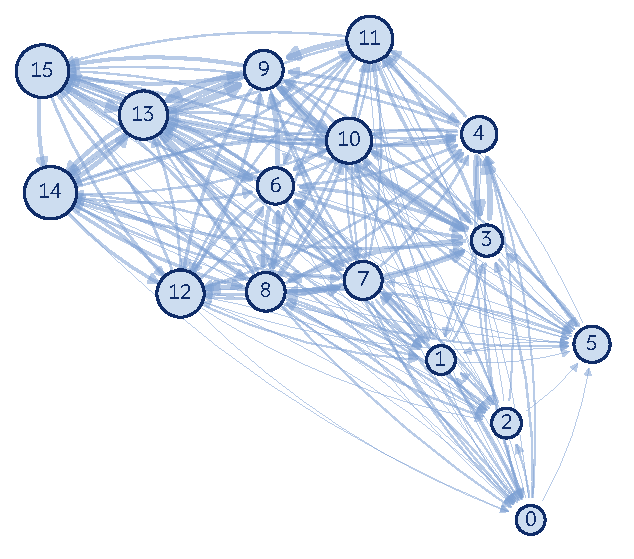
\includegraphics[height=0.66\textheight]{figs/belgium_requests.pdf}
\column{0.5\textwidth}
\begin{itemize}\setlength{\itemsep}{5pt}
\item спрос получен гравитационной моделью: крупные города обмениваются большими объёмами
\item толщина стрелки --- объём $d_k$: от части вместимости машины до нескольких машин
\item одна машина перевозит груз \emph{разных} заявок: заявки, проходящие по одному ребру, используют общие рейсы
\end{itemize}
\medskip
\begin{alertblock}{Основной вопрос}
когда выгоднее прямая перевозка, а когда --- консолидация груза на промежуточном складе и отправка полной машиной?
\end{alertblock}
\end{columns}
\end{frame}

\begin{frame}{Особенность 1: оплачивается рейс, а не объём груза}
\begin{columns}[T]
\column{0.5\textwidth}
\centering
\begin{tikzpicture}
\begin{axis}[width=0.95\linewidth,height=5.2cm,xlabel={объём на ребре $e$},ylabel={стоимость ребра $e$},
  xtick={0,50,100,150},xticklabels={0,$C$,$2C$,$3C$},ytick={1,2,3},yticklabels={$c_e$,$2c_e$,$3c_e$},
  ymin=0,ymax=3.5,xmin=0,xmax=165,axis lines=left,clip=false,label style={font=\small},tick label style={font=\small}]
\addplot[const plot mark right,line width=2pt,cStep] coordinates {(0,0)(0.01,1)(50,1)(50.01,2)(100,2)(100.01,3)(150,3)};
\addplot[dashed,hseGray,thick] coordinates {(0,0)(150,3)} node[pos=1,right,font=\scriptsize,text=hseGray,align=left] {линейная\\модель};
\node[font=\scriptsize,text=cStep,align=left,anchor=south west] at (axis cs:4,2.45) {$C{+}1$ единица:\\ещё одна машина};
\draw[-{Latex[length=1.5mm]},cStep,thick] (axis cs:34,2.42) -- (axis cs:50,2.08);
\end{axis}
\end{tikzpicture}
\column{0.5\textwidth}
\begin{block}{Стоимость ребра --- ступенчатая функция}
\[
\text{cost}_e(x)=c_e\left\lceil \frac{x}{C}\right\rceil
\]
\end{block}
\begin{itemize}
\item функция \textbf{разрывная и невыпуклая}, общая для всех заявок на ребре: решение для одной заявки зависит от остальных
\item перевозка $51$ единицы стоит столько же, сколько две полные машины, а дозагрузка неполной машины \textbf{не увеличивает стоимость}
\item классические алгоритмы (поток минимальной стоимости, кратчайшие пути) предполагают линейную стоимость и здесь неприменимы
\end{itemize}
\end{columns}
\end{frame}

\begin{frame}{Особенность 2: ограниченная ёмкость складов}
\begin{columns}[T]
\column{0.46\textwidth}
\centering
\begin{tikzpicture}[scale=0.72]
  \node[storage,minimum size=13mm,fill=cCap!50,font=\normalsize] (h) at (0,0) {$v$};
  \foreach \a/\c in {150/cN1,180/cN2,210/cOK} {\draw[flow,draw=\c] (\a:2.3) -- (h);}
  \foreach \a/\c in {30/cN1,0/cN2,-30/cOK} {\draw[flow,draw=\c] (h) -- (\a:2.3);}
  \draw[flow,draw=hseGray,dashed] (-2.4,-1.7) -- (-1.0,-1.0);
  \node[lbl,text=hseGray,align=left,anchor=north] at (-1.3,-1.85) {склад заполнен:\\другой маршрут};
  \draw[thick,hseBlue] (2.9,-0.9) rectangle (3.3,0.9);
  \fill[cCap!70] (2.9,-0.9) rectangle (3.3,0.9);
  \node[lbl,right] at (3.4,0.9) {$W_v$};
  \node[lbl,right,align=left] at (3.4,0.1) {транзит\\$=W_v$};
  \node[lbl,right,text=cCap] at (3.4,-0.75) {$\ovl_v=1$};
\end{tikzpicture}

\medskip
{\small загрузка склада в решении:\\
$\ovl_v = \dfrac{\text{транзит через }v}{W_v}$,\quad $1$ --- склад заполнен}
\column{0.54\textwidth}
\begin{block}{Транзит через склад ограничен}
\[
\sum_{k:\,v\neq s_k,t_k} \bigl(\text{поток $k$ через $v$}\bigr) \le \textcolor{cCap}{W_v}\quad\forall v
\]
\end{block}
\begin{itemize}
\item после заполнения склада оставшийся транзит направляется через другие склады или по другим маршрутам
\item отправка и приём в пунктах $s_k$, $t_k$ перегрузом не считаются: прямой рейс $s_k\!\to\!t_k$ не расходует ёмкость складов
\end{itemize}
\end{columns}
\end{frame}

\begin{frame}{Модельный пример: обе особенности одновременно}
\centering
\begin{tikzpicture}[scale=0.9]
  \begin{scope}
  \node[storage] (a) at (0,1.3) {$a$};
  \node[storage] (b) at (0,-1.3) {$b$};
  \node[storage] (t) at (3.2,0) {$t$};
  \draw[flow] (a) -- node[lbl,above,sloped] {20 ед., 1 машина} (t);
  \draw[flow] (b) -- node[lbl,below,sloped] {20 ед., 1 машина} (t);
  \node[font=\small,align=center] at (1.6,-2.5) {\textbf{напрямую}\\$100+100=\mathbf{200}$};
  \end{scope}
  \begin{scope}[xshift=5.2cm]
  \node[storage] (a) at (0,1.3) {$a$};
  \node[storage,fill=cOK!25] (b) at (0,-1.3) {$b$};
  \node[storage] (t) at (3.2,0) {$t$};
  \draw[flow,draw=cOK] (a) -- node[lbl,left] {20} (b);
  \draw[flow,draw=cOK] (b) -- node[lbl,below,sloped] {40 ед., 1 машина} (t);
  \node[font=\small,align=center] at (1.6,-2.5) {\textbf{через склад $b$}\\$20+100+20\cdot1=\mathbf{140}$};
  \end{scope}
  \begin{scope}[xshift=10.4cm]
  \node[storage] (a) at (0,1.3) {$a$};
  \node[storage,fill=cCap!40] (b) at (0,-1.3) {$b$};
  \node[storage] (t) at (3.2,0) {$t$};
  \draw[flow,draw=cCap] (a) -- node[lbl,left] {10} (b);
  \draw[flow,draw=cCap] (a) -- node[lbl,above,sloped] {10} (t);
  \draw[flow,draw=cCap] (b) -- node[lbl,below,sloped] {30} (t);
  \node[font=\small,align=center] at (1.6,-2.5) {\textbf{если $W_b=10$}\\$20+100+100+10=230$:\\выгоднее прямая перевозка};
  \end{scope}
\end{tikzpicture}

\medskip
{\small $C=50$;\quad рейс $a\!\to\!t$ и $b\!\to\!t$ стоит 100, $a\!\to\!b$ --- 20;\quad перегруз $f_b=1$ за единицу.\par}
\takeaway{Консолидация экономит 30\%, но одно ограничение ёмкости склада отменяет выигрыш. В реальной сети таких альтернатив тысячи, и они взаимозависимы.}
\end{frame}

% ===========================================================================
\section{Потоки в сетях: от одного товара к многим}

\begin{frame}{Напоминание: поток минимальной стоимости}
\begin{columns}[T]
\column{0.52\textwidth}
Один товар, ориентированный граф $G=(V,E)$, на ребре пропускная способность $u_e$ и цена \emph{за единицу} $c_e$; $b_v$ --- предложение ($>0$) или спрос ($<0$) в вершине.
\begin{block}{LP-постановка}
\vspace{-6pt}
\begin{align*}
\min\ & \sum_{e\in E} c_e x_e\\
\text{при}\ & \sum_{e\in\delta^+(v)}x_e-\sum_{e\in\delta^-(v)}x_e=b_v\quad\forall v\\
& 0\le x_e\le u_e\quad\forall e
\end{align*}
\end{block}
\column{0.45\textwidth}
\begin{itemize}\setlength{\itemsep}{4pt}
\item матрица ограничений --- \textbf{матрица инцидентности} графа (лекция 2): она вполне унимодулярна
\item значит, при целых $u_e$, $b_v$ у LP есть \textbf{целое оптимальное решение} --- требование целочисленности не усложняет задачу
\item решается за полиномиальное время: сетевой симплекс, алгоритмы сокращения циклов отрицательной стоимости
\item частные случаи: кратчайший путь, максимальный поток, задача о назначениях
\end{itemize}
\end{columns}
\end{frame}

\begin{frame}{Многопродуктовый поток (Multi-Commodity Flow)}
\begin{columns}[T]
\column{0.5\textwidth}
Теперь заявок много: $k=(s_k,t_k,d_k)$, и все они делят пропускную способность рёбер.
\begin{block}{Постановка на рёбрах (arc-based)}
\vspace{-6pt}
\begin{align*}
\min\ & \sum_{k\in K}\sum_{e\in E} c_e x^k_e\\
\text{при}\ & \sum_{e\in\delta^+(v)}x^k_e-\sum_{e\in\delta^-(v)}x^k_e=
\begin{cases} d_k & v=s_k\\ -d_k & v=t_k\\ 0&\text{иначе}\end{cases}\\
& \sum_{k\in K} x^k_e\le u_e\quad\forall e\qquad x\ge 0
\end{align*}
\end{block}
\column{0.47\textwidth}
\begin{itemize}\setlength{\itemsep}{4pt}
\item общие ограничения $\sum_k x^k_e\le u_e$ \textbf{связывают} заявки, вполне унимодулярность пропадает
\item LP по-прежнему решается полиномиально, но оптимум может быть \alert{дробным}
\item целочисленный MCF NP-труден уже для двух товаров
\item переменных $|K|\cdot|E|$: при $|V|=150$ и полном графе --- сотни миллионов
\end{itemize}
\takeaway{Без ограничений пропускной способности задача распалась бы на $|K|$ независимых кратчайших путей.}
\end{columns}
\end{frame}

\begin{frame}{Постановка на путях (path-based)}
\begin{columns}[T]
\column{0.5\textwidth}
$\Pi_k$ --- все пути из $s_k$ в $t_k$, $x^k_p\ge0$ --- поток заявки $k$ по пути $p$, $c_p=\sum_{e\in p}c_e$.
\begin{block}{Модель на путях}
\vspace{-6pt}
\begin{align*}
\min\ & \sum_{k\in K}\sum_{p\in\Pi_k} c_p\,x^k_p\\
\text{при}\ & \sum_{p\in\Pi_k} x^k_p = d_k \quad\forall k &&(\sigma_k)\\
& \sum_{k\in K}\sum_{p\in\Pi_k:\,e\in p} x^k_p \le u_e\quad\forall e &&(\pi_e\le 0)
\end{align*}
\end{block}
\column{0.47\textwidth}
\begin{itemize}\setlength{\itemsep}{4pt}
\item \textbf{теорема о декомпозиции потока}: любой поток заявки раскладывается на потоки по путям и циклам; без циклов модели эквивалентны
\item ограничений всего $|K|+|E|$, баланс в вершинах выполняется автоматически
\item зато путей \alert{экспоненциально много}
\item в оптимуме LP базисных переменных не больше числа ограничений: поток распределён по \textbf{небольшому числу} путей
\end{itemize}
\takeaway{Перечислять все пути не требуется: достаточно находить пути, улучшающие решение.}
\end{columns}
\end{frame}

% ===========================================================================
\section{Целочисленное программирование}

\begin{frame}{Линейное программирование (LP): напоминание}
\begin{columns}[T]
\column{0.5\textwidth}
\textbf{Задача LP}: переменные --- вещественные числа, цель и ограничения --- линейные
\[
\begin{aligned}
\max\ & 3x_1+2x_2\\
\text{при}\ & x_1+x_2\le 4{,}5\\
& 2x_1 + x_2 \le 7\\
& x_1,\,x_2\ge 0
\end{aligned}
\]
\begin{itemize}
\item допустимое множество --- многогранник, оптимум --- в его вершине
\item эффективные методы: симплекс-метод, методы внутренней точки; задачи с миллионами переменных решаются за приемлемое время
\end{itemize}
\column{0.5\textwidth}
\centering
\begin{tikzpicture}[scale=0.85]
  \draw[-{Latex},thick] (0,0) -- (5.3,0) node[below] {$x_1$};
  \draw[-{Latex},thick] (0,0) -- (0,5.3) node[left] {$x_2$};
  \foreach \i in {1,...,4} {\draw (\i,0.08)--(\i,-0.08) node[below,font=\scriptsize] {\i}; \draw (0.08,\i)--(-0.08,\i) node[left,font=\scriptsize] {\i};}
  \fill[hsePale] (0,0) -- (3.5,0) -- (2.5,2) -- (0,4.5) -- cycle;
  \draw[hseLightBlue,thick] (0,0) -- (3.5,0) -- (2.5,2) -- (0,4.5) -- cycle;
  \fill[cCap] (2.5,2) circle (2.5pt) node[above right,font=\scriptsize,text=cCap] {LP: $(2{,}5;\ 2)$, цель $11{,}5$};
  \draw[-{Latex},thick,cOK] (1,1) -- ++(0.9,0.6) node[right,font=\scriptsize] {рост цели};
  \foreach \x in {0,...,4} \foreach \y in {0,...,4} {\fill[hseGray!60] (\x,\y) circle (1.3pt);}
\end{tikzpicture}
\end{columns}
\end{frame}

\begin{frame}{Целочисленное программирование (MILP)}
\begin{columns}[T]
\column{0.5\textwidth}
\centering
\begin{tikzpicture}[scale=0.85]
  \draw[-{Latex},thick] (0,0) -- (5.3,0) node[below] {$x_1$};
  \draw[-{Latex},thick] (0,0) -- (0,5.3) node[left] {$x_2$};
  \foreach \i in {1,...,4} {\draw (\i,0.08)--(\i,-0.08) node[below,font=\scriptsize] {\i}; \draw (0.08,\i)--(-0.08,\i) node[left,font=\scriptsize] {\i};}
  \fill[hsePale!60] (0,0) -- (3.5,0) -- (2.5,2) -- (0,4.5) -- cycle;
  \draw[hseLightBlue,thick,dashed] (0,0) -- (3.5,0) -- (2.5,2) -- (0,4.5) -- cycle;
  \foreach \x/\y in {0/0,1/0,2/0,3/0,0/1,1/1,2/1,3/1,0/2,1/2,2/2,0/3,1/3,0/4} {\fill[hseBlue] (\x,\y) circle (2pt);}
  \fill[cCap] (2.5,2) circle (2.5pt) node[above right,font=\scriptsize,text=cCap] {LP: $11{,}5$, дробное};
  \draw[cOK,very thick] (3,1) circle (4pt);
  \node[font=\scriptsize,text=cOK,align=left,anchor=west] at (3.2,1.0) {целый оптимум\\$(3;\ 1)$: $11$};
  \draw[hseGray,thick] (2,2) circle (4pt);
  \node[font=\scriptsize,text=hseGray,anchor=east] at (1.85,2.25) {$(2;\ 2)$: $10$};
\end{tikzpicture}
\source{округление LP-решения не даёт оптимума: $(3;\ 2)$ недопустима, а $(2;\ 2)$ даёт только 10}
\column{0.5\textwidth}
\begin{block}{MILP: часть переменных целые}
\[
\min\ c^\top x\quad\text{при}\ Ax\le b,\ \ x_j\in\Int\ \ \text{для } j\in J
\]
\end{block}
\begin{itemize}
\item целые переменные --- это \textbf{количества} (машины, смены) и \textbf{решения да/нет} (открыть склад)
\item задача \textbf{NP-трудна}; LP-релаксация (отказ от требования целочисленности) даёт лишь нижнюю оценку
\item исключение --- вполне унимодулярные матрицы, как у потока одного товара
\end{itemize}
\end{columns}
\end{frame}

\begin{frame}{Линеаризация: машины как целые переменные}
\begin{columns}[T]
\column{0.5\textwidth}
Нелинейная целевая функция $\sum_e c_e\lceil f_e/C\rceil$ не допускается в MILP. Введём
\begin{itemize}
\item $f_e\in\Real_+$ --- суммарный поток по ребру $e$
\item $y_e\in\Int_+$ --- число машин на ребре $e$
\end{itemize}
\begin{block}{Линейная запись ступенчатой стоимости}
\[
\min\ \sum_{e} c_e\,y_e\quad\text{при}\quad f_e\le C\,y_e,\ \ y_e\in\Int_+
\]
\end{block}
\column{0.47\textwidth}
\begin{itemize}\setlength{\itemsep}{4pt}
\item при минимизации решатель выбирает наименьшее допустимое $y_e$, то есть $y_e=\lceil f_e/C\rceil$
\item $C=10$, $c_e=500$, $f_e=23$: $y_e\ge2{,}3$ $\Rightarrow$ $y_e=3$, цена 1500
\item в LP-релаксации $y_e=f_e/C$: ступенчатая функция заменяется линейной, \alert{консолидация перестаёт давать выигрыш}, и нижняя оценка оказывается слабой
\end{itemize}
\takeaway{Целые $y_e$ делают модель линейной, но превращают LP в MILP.}
\end{columns}
\end{frame}

\begin{frame}{Наша модель целиком: потоки на рёбрах}
\footnotesize
$x^k_e\in\Real_+$ --- поток заявки $k$ по ребру $e$;\quad $y_e\in\Int_+$ --- число машин на $e$
\vspace{-6pt}
\begin{align*}
\min\;& \textcolor{cStep}{\sum_{e\in E} c_e\,y_e}
 \;+\;\sum_{k\in K}\ \sum_{\substack{v\in V\\ v\neq s_k,t_k}}\ \sum_{e\in\delta^-(v)} f_v\,x^k_e
 &&\text{рейсы $+$ перегрузы}\\[-2pt]
\text{при}\;&
\sum_{e\in\delta^+(v)} x^k_e-\sum_{e\in\delta^-(v)} x^k_e=
 \begin{cases} d_k & v=s_k\\ -d_k & v=t_k\\ 0 & \text{иначе}\end{cases}
 && \forall k,\ \forall v \quad\text{(сохранение потока)}\\[-2pt]
&\textcolor{cStep}{\sum_{k\in K} x^k_e\le C\,y_e} && \forall e\in E \quad\text{(достаточно машин)}\\
&\textcolor{cCap}{\sum_{k\in K:\,v\neq s_k,t_k}\ \sum_{e\in\delta^-(v)} x^k_e \le W_v} && \forall v\in V \quad\text{(ёмкость склада)}\\
& x\ge 0,\quad y\in\Int_+^{|E|}
\end{align*}
{\small переменных $|K|\cdot|E|+|E|$, где $|E|=|V|(|V|-1)$ (граф достроен до полного):
$\approx6\cdot10^3$ при 10 складах, $\approx3{,}7\cdot10^8$ при 150\par}
\vspace{2pt}
\source{В конкурсе 2026 года вместо $W_v$ --- отдельные ёмкости $U^-_v$ на приём и $U^+_v$ на отправку: см.~\texttt{2026/optimal-logistic-network-contest/MCF\_ext.md}}
\end{frame}

\begin{frame}{Та же модель на путях}
\footnotesize
$\Pi_k$ --- все пути из $s_k$ в $t_k$;\quad $x^k_p\in\Real_+$ --- поток заявки $k$ по пути $p\in\Pi_k$;\quad $y_e\in\Int_+$ --- как раньше
\vspace{-6pt}
\begin{align*}
\min\;& \textcolor{cStep}{\sum_{e\in E} c_e\,y_e}
 \;+\;\sum_{k\in K}\ \sum_{p\in\Pi_k}\ \sum_{\substack{v\in p\\ v\neq s_k,t_k}} f_v\,x^k_p
 &&\text{рейсы $+$ перегрузы}\\[-2pt]
\text{при}\;& \sum_{p\in\Pi_k} x^k_p = d_k && \forall k \quad\text{(спрос)}\\[-2pt]
&\textcolor{cStep}{\sum_{k\in K}\ \sum_{p\in\Pi_k:\,e\in p} x^k_p\le C\,y_e} && \forall e\in E \quad\text{(достаточно машин)}\\[-2pt]
&\textcolor{cCap}{\sum_{k\in K}\ \sum_{p\in\Pi_k:\,v\in p,\ v\neq s_k,t_k} x^k_p \le W_v} && \forall v\in V \quad\text{(ёмкость склада)}
\end{align*}
\vspace{-8pt}
\begin{columns}[T]
\column{0.55\textwidth}
\begin{itemize}\setlength{\itemsep}{2pt}
\item переменных $\sum_k|\Pi_k|+|E|$: путей экспоненциально много, но в~решении поток распределён по небольшому числу путей
\item решаем модель на небольшом \textbf{пуле путей} $P_k\subset\Pi_k$ --- так устроен и алгоритм GVNS дальше
\end{itemize}
\column{0.45\textwidth}
\textbf{Без целочисленности} каждый путь имеет собственную стоимость единицы груза:
\[
\frac1C\sum_{e\in p} c_e+\!\!\sum_{\substack{v\in p\\ v\neq s_k,t_k}}\!\! f_v
\]
выгодны прямые пути без перегрузов
\end{columns}
\end{frame}

\begin{frame}{Модель на путях: решатель выбирает комбинацию}
\begin{columns}[T]
\column{0.44\textwidth}
\centering
\begin{tikzpicture}[scale=0.95,
  dir/.style={-{Latex[length=2mm]},thick,dashed},
  hub/.style={-{Latex[length=2mm]},line width=1.6pt}]
  \node[storage] (a) at (0,1.5) {$a$};
  \node[storage] (b) at (0,0) {$b$};
  \node[storage] (c) at (0,-1.5) {$c$};
  \node[storage] (t) at (4.6,0) {$t$};
  \node[storage,fill=cCap!20] (h) at (2.6,-2.6) {$h$};
  \draw[dir,cN1] (a) -- (t);
  \draw[dir,cN2] (b) -- (t);
  \draw[dir,cStep] (c) -- (t);
  \draw[hub,cN1] (a) to[bend left=22] (h);
  \draw[hub,cN2] (b) to[bend left=8] (h);
  \draw[hub,cStep] (c) -- (h);
  \draw[hub,hseBlue] (h) -- node[lbl,right,pos=0.4,align=left,xshift=1mm] {общая\\машина} (t);
  \node[font=\scriptsize,text=cN1,anchor=east] at (a.west) {$d_1=4$};
  \node[font=\scriptsize,text=cN2,anchor=east] at (b.west) {$d_2=5$};
  \node[font=\scriptsize,text=cStep,anchor=east] at (c.west) {$d_3=6$};
\end{tikzpicture}
\source{пул каждой заявки: \emph{прямой путь} (пунктир) и \emph{через склад $h$};\\
$C=10$;\ рейс в $t$ --- 100, в $h$ --- 30;\ $f_h=1$,\ $W_h=10$}
\column{0.56\textwidth}
\footnotesize
\setlength{\tabcolsep}{4pt}
\begin{tabular}{@{}lccr@{}}
\toprule
через $h$ & груз в $h$ & $\le W_h$? & стоимость\\
\midrule
никто & 0 & $\checkmark$ & 300\\
только \textcolor{cN1}{1} & 4 & $\checkmark$ & 334\\
\textcolor{cN1}{1} и \textcolor{cStep}{3} & 10 & $\checkmark$ & 270\\
\textbf{\textcolor{cN1}{1} и \textcolor{cN2}{2}} & \textbf{9} & $\checkmark$ & \textcolor{cOK}{\textbf{269}}\\
\textcolor{cN2}{2} и \textcolor{cStep}{3} & 11 & \textcolor{cCap}{$\times$} & ---\\
все три & 15 & \textcolor{cCap}{$\times$} & ---\\
\bottomrule
\end{tabular}

\medskip
\begin{itemize}\setlength{\itemsep}{2pt}
\item по отдельности путь через $h$ невыгоден ни одной заявке: $334>300$
\item выгодна только \textbf{комбинация}: две заявки делят машину $h\to t$
\item ёмкость $W_h$ отсекает часть комбинаций
\item комбинаций $\prod_k|P_k|$; решатель не перебирает их, а~находит наилучшую методом ветвей и границ
\end{itemize}
\end{columns}
\end{frame}

\begin{frame}{Метод ветвей и границ}
\begin{columns}[T]
\column{0.56\textwidth}
\centering
\begin{tikzpicture}[level distance=17mm,
  level 1/.style={sibling distance=45mm},
  edge from parent/.style={draw=hseBlue!60,thick}]
\node[bbnode] {корень, LP: $11{,}5$\\$(2{,}5;\ 2)$ --- дробное}
  child {node[bbnode,fill=hseLightGray!60] {$x_1\le2$\\LP: $11$ в $(2;\ 2{,}5)$\\не лучше рекорда:\\\textbf{отсечено}}
}
  child {node[bbnode,fill=hsePaleGreen] {$x_1\ge3$\\LP: $11$ в $(3;\ 1)$\\целое: \textbf{рекорд}}
};
\end{tikzpicture}
\source{граница $11$ $=$ рекорд $11$: оптимальность доказана}
\column{0.44\textwidth}
\begin{enumerate}\setlength{\itemsep}{3pt}
\item решаем LP; дробное $x_j=v$ --- \textbf{ветвление}: $x_j\le\lfloor v\rfloor$ или $x_j\ge\lceil v\rceil$
\item лучшее целое решение --- \textbf{рекорд}
\item ветка с LP-оценкой не лучше рекорда \textbf{отсекается}
\end{enumerate}
\medskip
\begin{block}{Две границы и зазор}
рекорд $\bar z$ и двойственная граница $\underline z$:
\[
\text{оптимум}\in[\underline z,\ \bar z],\qquad gap=\frac{\bar z-\underline z}{\underline z}
\]
\end{block}
\end{columns}
\takeaway{Решатель, остановленный по лимиту времени, остаётся полезен: рекорд --- допустимое решение, $\underline z$ --- гарантия.}
\end{frame}

\begin{frame}[fragile]{Решатели и средства моделирования}
\begin{columns}[T]
\column{0.40\textwidth}
\small
\textbf{Открытые}: HiGHS, SCIP, CBC\\
\textbf{Коммерческие}: Gurobi, CPLEX, Xpress, COPT\\[3pt]
\textbf{Моделирование}: PuLP, Pyomo, OR-Tools (Python), JuMP (Julia)

\begin{itemize}
\item модель описывается декларативно, алгоритм решения выбирает решатель
\item в проекте: \textbf{HiGHS} через PuLP --- и точный метод для сравнения, и вычислительное ядро эвристики
\end{itemize}
\column{0.60\textwidth}
\begin{beamercolorbox}[rounded=true,sep=3pt]{block body}
\fontsize{6.6}{7.6}\selectfont
\begin{semiverbatim}
import pulp
m = pulp.LpProblem("net", pulp.LpMinimize)
x = \{(k, p): pulp.LpVariable(f"x_\{k\}_\{i\}", lowBound=0)
     for k in K for i, p in enumerate(paths[k])\}
y = \{e: pulp.LpVariable(f"y_\{e\}", lowBound=0, cat="Integer")
     for e in E\}
m += (pulp.lpSum(c[e] * y[e] for e in E)            \# рейсы
    + pulp.lpSum(f[v] * x[k, p] for (k, p) in x
                 for v in p[1:-1]))                 \# перегрузы
for k in K:                                         \# спрос
    m += pulp.lpSum(x[k, p] for p in paths[k]) == d[k]
for e in E:                                         \# машины
    m += pulp.lpSum(x[k, p] for (k, p) in x
                    if e in edges(p)) <= C * y[e]
for v in V:                                         \# ёмкость
    m += pulp.lpSum(x[k, p] for (k, p) in x
                    if v in p[1:-1]) <= W[v]
m.solve(pulp.HiGHS(timeLimit=60, gapRel=0.01))
\end{semiverbatim}
\end{beamercolorbox}
\source{упрощённый фрагмент \texttt{Solver.py} проекта: модель на путях}
\end{columns}
\end{frame}

\begin{frame}{Пределы применимости MILP-решателей}
\begin{columns}[T]
\column{0.5\textwidth}
\begin{itemize}\setlength{\itemsep}{4pt}
\item HiGHS и SCIP, от 30 минут до 4 часов на сеть: \textbf{ни одна} из 50 сетей не решена с доказанной оптимальностью
\item до $|V|\approx 40$ рекорд решателя близок к оптимуму, а двойственная граница точна
\item $|V|=45$--$59$: SCIP не находит ни одного допустимого решения, HiGHS --- только решения, которые эвристика улучшает на 14--58\%
\item $|V|\ge100$: модель \alert{не помещается в память}
\end{itemize}
\column{0.5\textwidth}
\begin{block}{Почему}
\begin{itemize}
\item $10^5$--$10^8$ непрерывных переменных и тысячи целых $y_e$
\item слабая LP-релаксация: ступенька становится прямой, отсечение ветвей малоэффективно
\item симметрии: много решений одинаковой стоимости
\end{itemize}
\end{block}
\takeaway{Решатель эффективен как подпрограмма для небольших подзадач и как источник нижней оценки.}
\end{columns}
\end{frame}

% ===========================================================================
\section{Большие задачи: классические подходы}

\begin{frame}{Генерация столбцов (column generation)}
\begin{columns}[T]
\column{0.5\textwidth}
\begin{enumerate}\setlength{\itemsep}{4pt}
\item \textbf{ограниченная задача} (restricted master): LP на малом пуле путей $P_k\subset\Pi_k$, например на кратчайших
\item берём двойственные переменные: $\sigma_k$ (спрос) и $\pi_e\le0$ (пропускная способность)
\item \textbf{задача ценообразования} (pricing): для каждой заявки ищем путь с отрицательной приведённой стоимостью
\item найденный путь добавляется в пул; если таких путей нет, LP решена оптимально \emph{на множестве всех путей}
\end{enumerate}
\column{0.47\textwidth}
\begin{block}{Приведённая стоимость пути}
\[
\bar c_p=\sum_{e\in p}\bigl(c_e-\pi_e\bigr)-\sigma_k
\]
\end{block}
\begin{itemize}
\item веса $c_e-\pi_e\ge0$ $\Rightarrow$ ценообразование --- \textbf{кратчайший путь} алгоритмом Дейкстры
\item загруженные рёбра (большое $|\pi_e|$) становятся дороже
\item для MILP --- внутри ветвей и границ: branch-and-price
\end{itemize}
\end{columns}
\takeaway{Пути порождаются по мере необходимости, поэтому их экспоненциальное число не препятствует решению.}
\end{frame}

\begin{frame}{Лагранжева релаксация}
\begin{columns}[T]
\column{0.52\textwidth}
Переносим связывающие ограничения $\sum_k x^k_e\le u_e$ в цель со штрафами $\lambda_e\ge0$:
\[
L(\lambda)=\min_{x\in X}\ \sum_{k}\sum_{e}(c_e+\lambda_e)\,x^k_e-\sum_e\lambda_e u_e
\]
\begin{itemize}
\item при фиксированных $\lambda$ задача распадается на $|K|$ \textbf{независимых} задач о кратчайшем пути, решаемых параллельно
\item $L(\lambda)\le\text{OPT}$ при любых $\lambda\ge0$ --- \textbf{нижняя оценка}
\item лучшая оценка: $\max_{\lambda\ge0}L(\lambda)$ --- вогнутая негладкая задача
\end{itemize}
\column{0.45\textwidth}
\begin{block}{Субградиентный метод}
\[
\lambda_e\leftarrow\max\Bigl(0,\ \lambda_e+t\Bigl(\sum_k x^k_e-u_e\Bigr)\Bigr)
\]
штраф на перегруженных рёбрах растёт, на недогруженных --- уменьшается
\end{block}
\begin{itemize}
\item требуется подбор шага $t$ и критерия остановки
\item решение $L(\lambda)$ обычно недопустимо; эвристика восстанавливает допустимость и даёт верхнюю оценку
\end{itemize}
\end{columns}
\end{frame}

\begin{frame}{Эвристики, агрегация и матэвристики}
\begin{columns}[T]
\column{0.5\textwidth}
\begin{itemize}\setlength{\itemsep}{4pt}
\item \textbf{жадные}: последовательная маршрутизация заявок по кратчайшим путям с учётом уже задействованных машин
\item \textbf{метаэвристики} --- общие схемы поиска, управляющие локальными эвристиками: имитация отжига, табу-поиск, генетические алгоритмы, \textbf{поиск с чередующимися окрестностями}
\item \textbf{агрегация}: укрупнить узлы, сгруппировать заявки с похожими $s_k,t_k$, решить грубую модель и уточнить
\end{itemize}
\source{быстро и масштабируемо, но без гарантий оптимальности}
\column{0.47\textwidth}
\begin{block}{Матэвристика (matheuristic)}
метаэвристика, внутри которой подзадачи решаются точными методами математического программирования
\end{block}
\begin{itemize}
\item эвристика выбирает \textbf{немного перспективных маршрутов} и тем сужает пространство поиска
\item MILP-решатель за короткое время точно решает задачу только на них
\item та же идея, что в генерации столбцов, но пути предлагаются эвристически
\end{itemize}
\source{Maniezzo, Stützle, Voß (ред.), 2009}
\end{columns}
\end{frame}

% ===========================================================================
\section{GVNS с MILP-решателем: матэвристика}

\begin{frame}{Поиск с чередующимися окрестностями (VNS)}
\begin{columns}[T]
\column{0.5\textwidth}
\centering
\begin{tikzpicture}
\begin{axis}[width=\linewidth,height=5cm,axis lines=left,xtick=\empty,ytick=\empty,
  xlabel={пространство решений},ylabel={стоимость},ymin=0,ymax=4.6,xmin=0,xmax=10,clip=false,label style={font=\small}]
\addplot[domain=0:10,samples=200,thick,hseBlue] {2.4+0.9*sin(deg(1.9*x))+0.6*sin(deg(0.7*x+1))-0.12*x};
\addplot[only marks,mark=*,mark size=2.5pt,cN1] coordinates {(2.35,1.17)};
\node[font=\scriptsize,text=cN1,anchor=north] at (axis cs:2.35,1.0) {локальный минимум в $N_1$};
\draw[-{Latex},thick,cN2] (axis cs:2.6,1.6) to[bend left=40] node[above,font=\scriptsize] {шаг в $N_2$, $N_3$} (axis cs:5.6,1.9);
\addplot[only marks,mark=*,mark size=2.5pt,cOK] coordinates {(8.95,0.86)};
\node[font=\scriptsize,text=cOK,anchor=north] at (axis cs:8.95,0.7) {лучше};
\end{axis}
\end{tikzpicture}
\column{0.5\textwidth}
\begin{itemize}\setlength{\itemsep}{4pt}
\item \textbf{окрестность} $N(x)$ --- решения, получаемые из $x$ одним элементарным преобразованием (ходом)
\item локальный минимум в одной окрестности часто не минимум в другой
\item \textbf{VND} (спуск): окрестности $N_1, N_2, N_3$ просматриваются по порядку; при улучшении поиск возвращается к $N_1$
\item \textbf{VNS}: в локальном минимуме выполняется \emph{встряска} (shaking) --- случайный шаг в $N_k$, --- после чего спуск повторяется
\item \textbf{GVNS} (General VNS) --- встряска $+$ полный VND (Hansen, Mladenović)
\end{itemize}
\end{columns}
\end{frame}

\begin{frame}{Решение --- это набор маршрутов}
\centering
\begin{tikzpicture}[node distance=5mm]
  \node[box,fill=hsePale,text width=4.0cm,font=\footnotesize] (gen) {\textbf{окрестность $N_i$}\\предлагает новые пути $Q$\\для каждой заявки};
  \node[box,right=of gen,text width=4.0cm,font=\footnotesize] (milp) {\textbf{MILP} на пуле $P\cup Q$:\\перераспределить потоки;\\лимит времени, зазор 1\%};
  \node[box,right=of milp,fill=hsePaleGreen,text width=4.0cm,font=\footnotesize] (keep) {стоимость снизилась:\\сохранить пути с потоком,\\удалить остальные};
  \node[box,below=2mm of keep,fill=hsePaleRed,text width=4.0cm,font=\footnotesize,minimum height=6mm] (drop) {иначе: отбросить $Q$};
  \draw[road] (gen) -- (milp);
  \draw[road] (milp) -- (keep);
  \draw[road] (milp.east) -- ++(0.25,0) |- (drop.west);
\end{tikzpicture}

\medskip
\begin{columns}[T]
\column{0.5\textwidth}
\begin{block}{Почему пути, а не потоки по рёбрам}
путь касается одной заявки, и \emph{добавить} путь в пул безопасно: старое решение остаётся допустимым, поэтому решение MILP не может ухудшиться
\end{block}
\column{0.5\textwidth}
\begin{itemize}
\item окрестности отличаются \textbf{только} генератором путей
\item начальное решение: все заявки на прямых рёбрах $s_k\!\to\!t_k$, машины округлены вверх
\item \textbf{эвристика предлагает пути, решатель выбирает их наилучшую комбинацию}
\end{itemize}
\end{columns}
\end{frame}

\begin{frame}[fragile]{GVNS в коде}
\begin{columns}[T]
\column{0.55\textwidth}
\begin{beamercolorbox}[rounded=true,sep=3pt]{block body}
\fontsize{7}{8.2}\selectfont
\begin{semiverbatim}
def solve(net, t_max):
    pool = \{k: [direct(k)] for k in K\}   \# старт
    sol = milp(pool)
    k = 1
    while k <= 3 and time() < t_max:
        shake(sol, N[k])          \# много случайных путей
        z0 = sol.cost
        vnd(sol)                  \# спуск N1 -> N2 -> N3
        k = 1 if sol.cost < z0 else k + 1

def try_move(sol, gen_paths):     \# общий шаг
    new = \{k: gen_paths(sol, k) for k in K\}
    cand = milp(sol.pool + new, warm=sol, limit=tau)
    if cand.cost < sol.cost:
        sol.accept(cand)          \# и чистит пустые пути
        return True
    return False
\end{semiverbatim}
\end{beamercolorbox}
\source{упрощённо по \texttt{VNS.py} проекта}
\column{0.45\textwidth}
\begin{itemize}\setlength{\itemsep}{4pt}
\item ход принимается \textbf{только при улучшении}, поэтому встряска не ухудшает рекорд
\item \textbf{встряска}: больше путей, случайный выбор, больший лимит времени MILP
\item \textbf{спуск}: 1--3 пути на заявку, лимит MILP 25--70 с
\item стоп: $k>3$ или $t_{\max}=2|V|$ минут
\end{itemize}
\end{columns}
\end{frame}

\begin{frame}{Вычислительный эксперимент: сеть Бельгии}
\begin{columns}[T]
\column{0.5\textwidth}
\centering
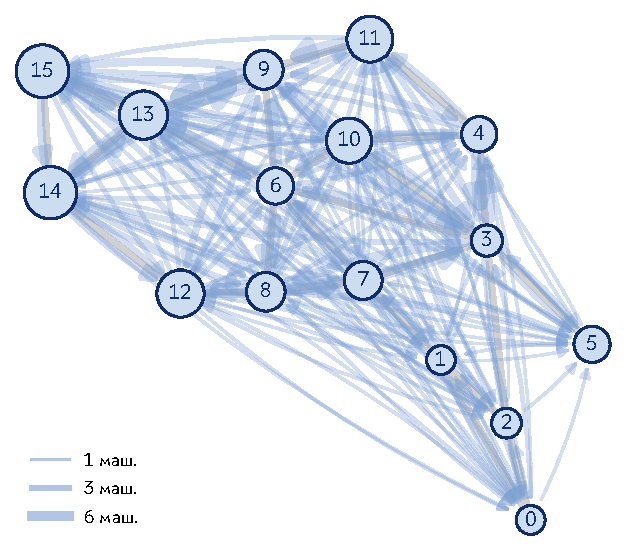
\includegraphics[height=0.68\textheight]{figs/belgium_start.pdf}
\source{стартовое решение: все заявки перевозятся напрямую; толщина --- число машин}
\column{0.5\textwidth}
Код проекта запускается на сети Бельгии ($|V|=16$, $|K|=180$):
\begin{enumerate}\setlength{\itemsep}{3pt}
\item \textbf{старт} $S_0$: все заявки напрямую
\item спуск только по $N_1$, пока он улучшает $\Rightarrow S_1$
\item из $S_1$ делаем \textbf{один} ход $N_2$ и, отдельно, \textbf{один} ход $N_3$
\end{enumerate}
\medskip
\small
\begin{tabular}{@{}lrrr@{}}
\toprule
 & стоимость & машин & загрузка машин\\
\midrule
$S_0$ & \SzeroPrice & \SzeroVeh & \SzeroFill\\
$S_1$ & \SonePrice & \SoneVeh & \SoneFill\\
\bottomrule
\end{tabular}
\end{columns}
\end{frame}

\begin{frame}{$N_1$: кратчайшие пути с учётом перегрузов}
\begin{columns}[T]
\column{0.5\textwidth}
\centering
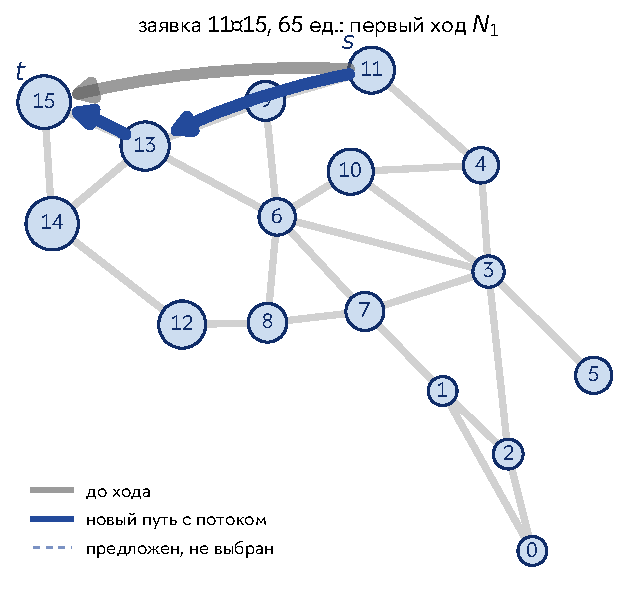
\includegraphics[width=\linewidth,height=0.72\textheight,keepaspectratio]{figs/n1_example.pdf}
\column{0.5\textwidth}
\begin{block}{Вспомогательный граф $G'$: цена единицы груза}
\[
c'_{vu}=f_v+f_u+\frac{c_{vu}}{C}
\]
\end{block}
\begin{itemize}\setlength{\itemsep}{3pt}
\item 20 кратчайших путей в $G'$ на заявку вычисляются заранее (алгоритм Йена); каждый ход добавляет из этого пула 1--3 новых пути
\item \NoneStory
\item первый ход из начального решения: \NoneFirstDelta, машин \NoneFirstVehFrom\ $\to$ \NoneFirstVehTo
\end{itemize}
\end{columns}
\end{frame}

\begin{frame}{$N_2$: дозагрузка неполных машин}
\begin{columns}[T]
\column{0.5\textwidth}
\centering
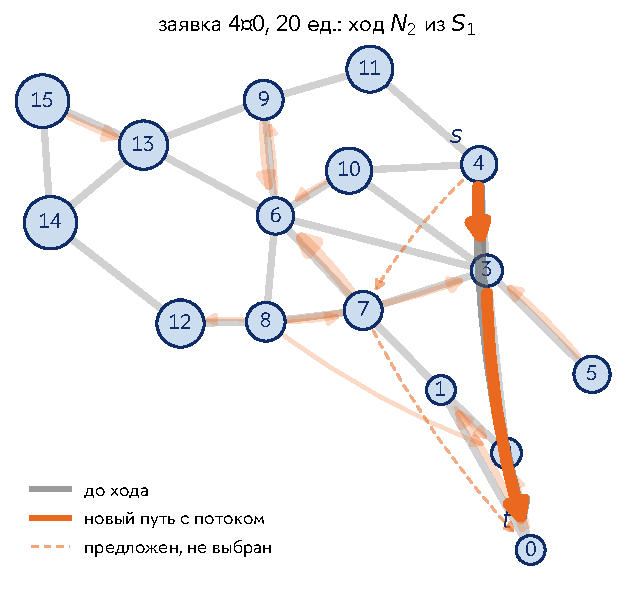
\includegraphics[width=\linewidth,height=0.72\textheight,keepaspectratio]{figs/n2_example.pdf}
\column{0.5\textwidth}
\begin{block}{Граф $G''$: свободное место дешевле}
\vspace{-4pt}
\begin{gather*}
\load_e=\Big(\textstyle\sum_k x^k_e\Big)\bmod C\\[-2pt]
c''_{vu}=f_v+f_u+\frac{\load_{vu}}{C}\Big(\frac{c_{vu}}{C}\Big)^{\!1/2}
\end{gather*}
чем меньше загружена последняя машина, тем дешевле ребро
\end{block}
\begin{itemize}\setlength{\itemsep}{2pt}
\item \NtwoStory
\item ход из $S_1$: \NtwoDelta; число машин уменьшилось на \NtwoLess\ рёбрах и выросло на \NtwoMore: поток перераспределён по всей сети
\end{itemize}
\end{columns}
\end{frame}

\begin{frame}{$N_3$: обход заполненного склада}
\begin{columns}[T]
\column{0.5\textwidth}
\centering
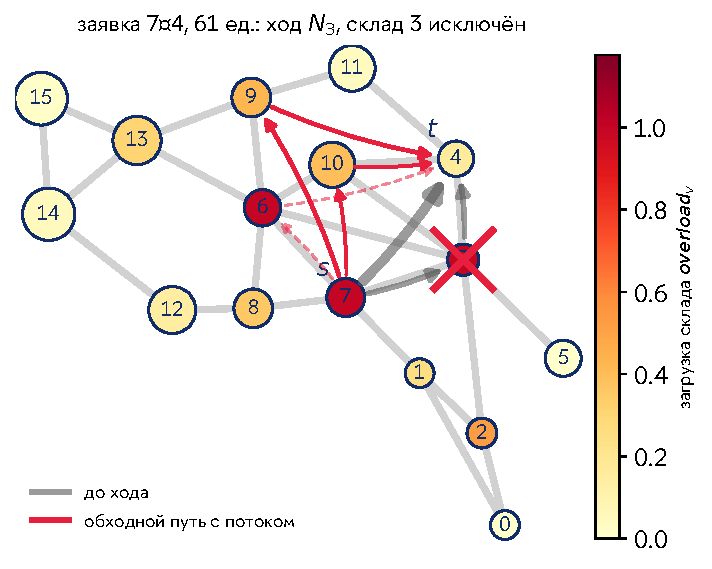
\includegraphics[width=\linewidth,height=0.72\textheight,keepaspectratio]{figs/n3_example.pdf}
\column{0.5\textwidth}
\begin{block}{Убрать из $G'$ самый загруженный склад}
\[
\ovl_v=\frac{\text{транзит через }v}{W_v}\ \to\ \max
\]
и найти новый кратчайший путь: обход через менее загруженные склады
\end{block}
\begin{itemize}\setlength{\itemsep}{2pt}
\item полный прогон GVNS, \NthreeAt-я минута: склады \NthreeFull\ заполнены; убираем склад \NthreeRemoved, транзит через него \NthreeTransit; \NthreeDelta
\item \NthreeStory
\item из $S_1$ --- \NthreeFromSone: там склады не заполнены
\end{itemize}
\end{columns}
\end{frame}

\begin{frame}{Три окрестности --- три разные задачи}
\centering
\small
\renewcommand{\arraystretch}{1.25}
\begin{tabular}{@{}>{\raggedright\arraybackslash}p{2.0cm}>{\raggedright\arraybackslash}p{3.6cm}>{\raggedright\arraybackslash}p{3.6cm}>{\raggedright\arraybackslash}p{3.6cm}@{}}
\toprule
 & \textcolor{cN1}{\textbf{$N_1$}} & \textcolor{cN2}{\textbf{$N_2$}} & \textcolor{cN3}{\textbf{$N_3$}}\\
\midrule
ищет & дешёвые пути с учётом перегрузов & рейсы, где есть свободное место & обходы заполненных складов\\
граф & $G'$, статичный & $G''$, строится по решению & $G'$ без склада\\
путей на заявку & 1--3 из пула & динамически & 1\\
результат на Бельгии & \SoneDelta\ за \SoneMoves\ хода из старта & \NtwoDelta\ за 1 ход из $S_1$ & \NthreeDelta\ за 1 ход, когда склады заполнены\\
\bottomrule
\end{tabular}

\medskip
\takeaway{Все три --- один и тот же примитив: генератор путей $\to$ MILP на пуле $\to$ принять, если дешевле.}
\end{frame}

\begin{frame}{Ход поиска: полный запуск GVNS на сети Бельгии}
\begin{columns}[T]
\column{0.62\textwidth}
\centering
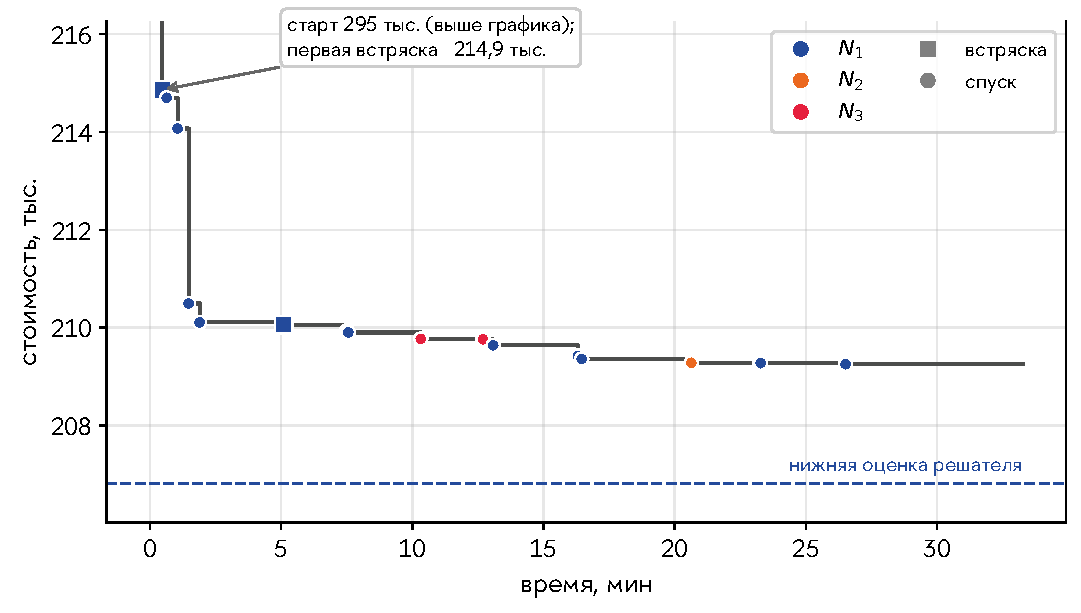
\includegraphics[width=\linewidth]{figs/convergence.pdf}
\column{0.38\textwidth}
\begin{itemize}\setlength{\itemsep}{4pt}
\item цвет принятого хода соответствует окрестности
\item первая встряска и спуск по $N_1$ дают основную часть снижения стоимости
\item затем улучшения дают $N_2$ и $N_3$: они меньше, но недостижимы в окрестности $N_1$
\item итог \TraceFinal\ за \TraceTime; нижняя оценка решателя \BelgiumDual, отклонение \BelgiumGap
\end{itemize}
\end{columns}
\end{frame}

% ===========================================================================
\section{Результаты}

\begin{frame}{Открытый набор: 50 сетей}
\begin{columns}[T]
\column{0.56\textwidth}
\begin{itemize}\setlength{\itemsep}{4pt}
\item генератор сетей (arXiv:2606.20653, данные на Zenodo, CC BY 4.0); каждая сеть воспроизводится по начальному числу (seed) генератора
\item \textbf{15 реальных геометрий}: дороги OpenStreetMap девяти стран Европы, пяти штатов США и Европейской России
\item \textbf{35 синтетических}: от 10 до 150 складов
\item реалистичная структура: размеры городов по закону Ципфа, гравитационный спрос, ёмкости складов по центральности (лекции о степенных законах и центральности)
\end{itemize}
\column{0.44\textwidth}
\centering
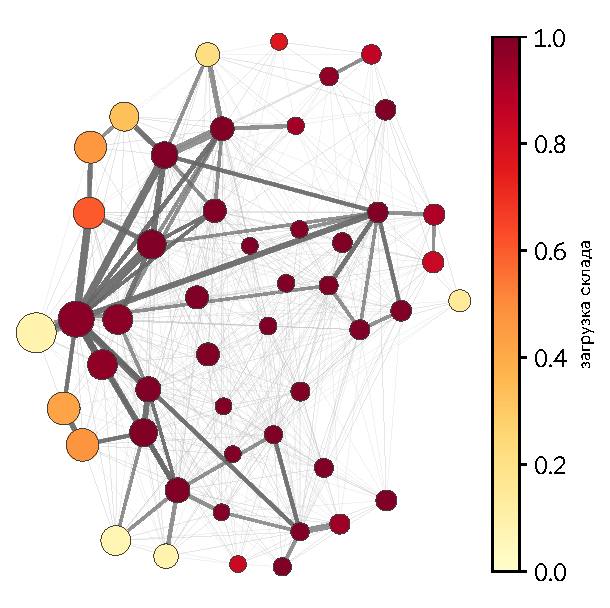
\includegraphics[height=0.6\textheight]{figs/germany_solution.pdf}
\source{Германия, 49 складов: решение GVNS. Цвет --- загрузка склада, толщина --- машины ($\ge3$)}
\end{columns}
\end{frame}

\begin{frame}{Как сравнивать, если оптимум неизвестен}
\centering
\begin{tikzpicture}[x=0.93cm]
  \draw[-{Latex[length=2.5mm]},thick,hseBlue] (0,0) -- (13.2,0) node[right,font=\scriptsize] {стоимость};
  \foreach \x/\lab/\col in {0.9/{LP-релаксация}/hseGray, 3.6/{граница\\решателя $\underline{z}$}/cN1, 6.2/{оптимум $z^\ast$\\(неизвестен)}/hseGray, 8.8/{GVNS}/hseOrange, 11.8/{рекорд\\решателя}/cOK}{
    \draw[thick,\col] (\x,-0.15) -- (\x,0.15);
    \node[font=\small,text=\col,align=center,above=1mm] at (\x,0.15) {\lab};
  }
  \draw[{Bar}-{Bar},thick,cN1] (3.6,-0.6) -- (8.8,-0.6) node[midway,below=3pt,font=\small,text=cN1] {$\gapLB$ --- не меньше истинного отклонения от оптимума};
\end{tikzpicture}

\medskip
\begin{columns}[T]
\column{0.5\textwidth}
\begin{block}{Две метрики}
$\gapLB=\dfrac{\mathit{GVNS}-\underline{z}}{\underline{z}}$ --- \textbf{гарантия} качества\\[4pt]
$\mathit{Ratio}=\dfrac{\text{метод}}{\mathit{GVNS}}$: больше 1 --- GVNS лучше
\end{block}
\column{0.5\textwidth}
\begin{itemize}
\item GVNS: 10 запусков на сеть, лимит $2|V|$ минут
\item решатель (HiGHS, контроль --- SCIP): от 30 минут до 4 часов --- сравнимый бюджет
\item суперкомпьютер НИУ ВШЭ cHARISMa, 8 ядер на задачу
\end{itemize}
\end{columns}
\end{frame}

\begin{frame}{Синтетические сети}
\begin{columns}[T]
\column{0.56\textwidth}
\centering
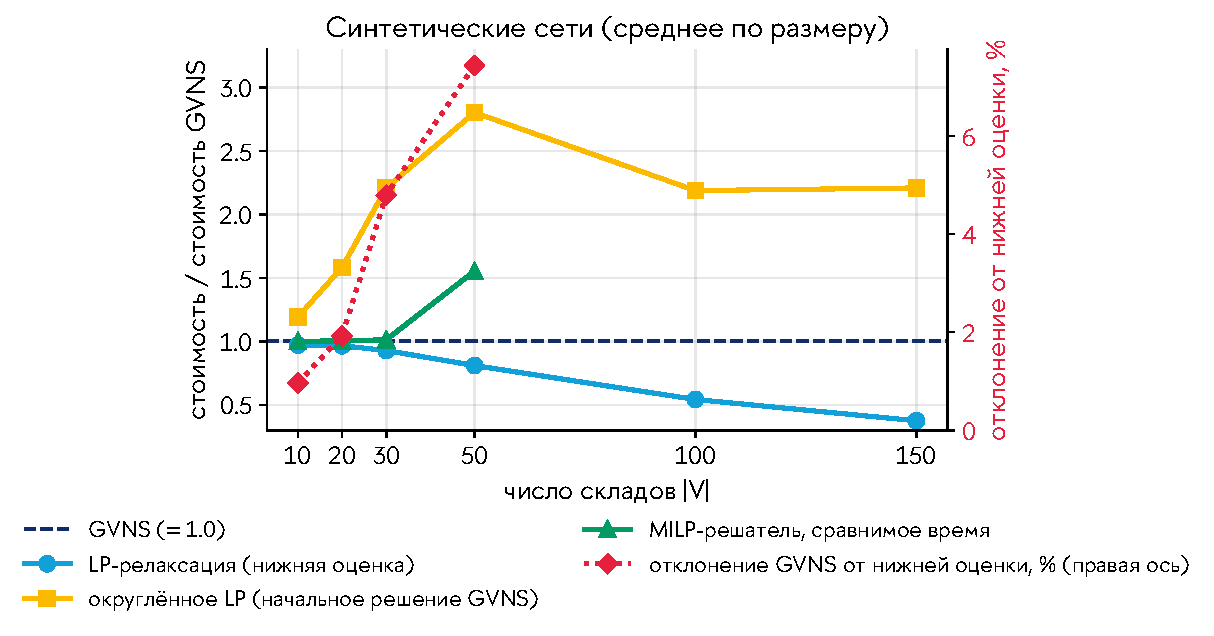
\includegraphics[width=0.94\linewidth]{figs/ratios_synthetic.pdf}
\column{0.44\textwidth}
\centering
\small
\setlength{\tabcolsep}{4pt}
\begin{tabular}{@{}rrcc@{}}
\toprule
$|V|$ & сетей & $\gapLB$ & выигрыш GVNS\\
\midrule
10  & 10 & 0{,}96\% & $\approx0$\%\\
20  & 7  & 1{,}92\% & 0{,}5\%\\
30  & 7  & 4{,}79\% & 1{,}3\%\\
50  & 5  & 7{,}44\% & \alert{32\%}\\
100 & 3  & --- & только GVNS\\
150 & 3  & --- & только GVNS\\
\bottomrule
\end{tabular}

\medskip
\raggedright
{\small до 20 складов GVNS в 1--2\% от гарантированной нижней оценки; на 50 складах решения GVNS в среднем \alert{на 32\% дешевле}, чем у решателя за сравнимое время (от 14\% до 58\% по сетям)\par}
\end{columns}
\end{frame}

\begin{frame}{Реальные дорожные сети}
\begin{columns}[T]
\column{0.58\textwidth}
\centering
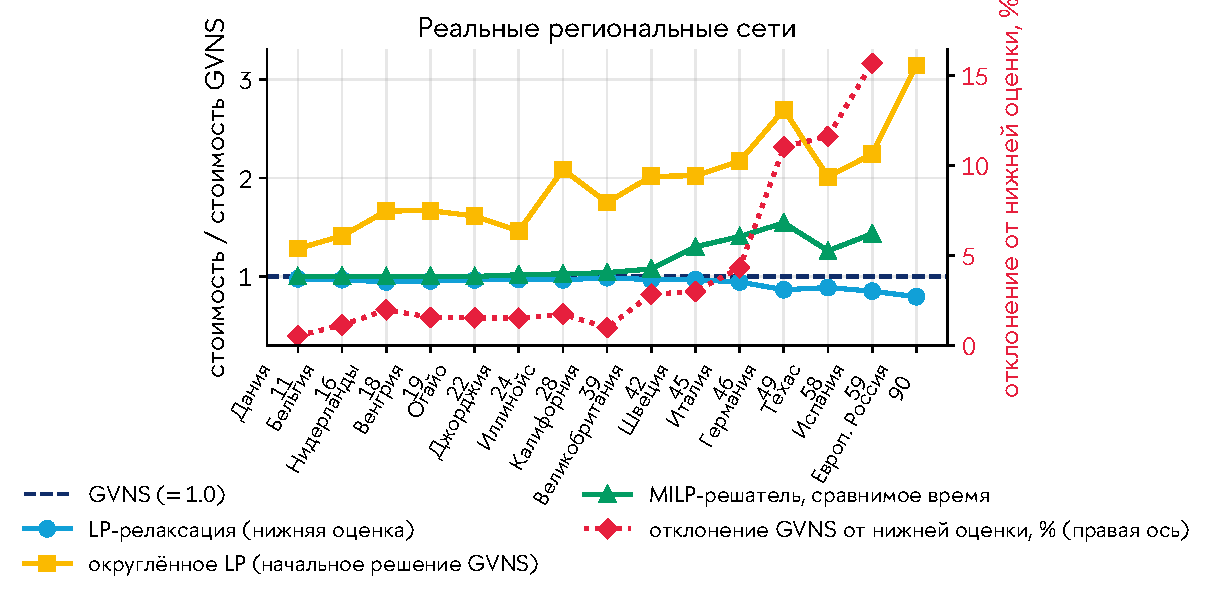
\includegraphics[width=\linewidth]{figs/ratios_real.pdf}
\column{0.42\textwidth}
\begin{itemize}\setlength{\itemsep}{4pt}
\item до 22 складов результаты GVNS и решателя близки; до Великобритании (42) GVNS дешевле на 2--7\%, от Швеции (45) до Испании (59) --- \alert{на 21--35\%}
\item $\gapLB$ от 0,5\% (Дания) до 15,7\% (Испания)
\item Европейская Россия (90 складов): GVNS --- единственный метод, давший решение; оно в 3,1 раза дешевле старта
\end{itemize}
\takeaway{Та же картина, что на синтетике: генератор воспроизводит трудность реальных сетей.}
\end{columns}
\end{frame}

\begin{frame}{Что даёт каждая окрестность}
\begin{columns}[T]
\column{0.56\textwidth}
\centering
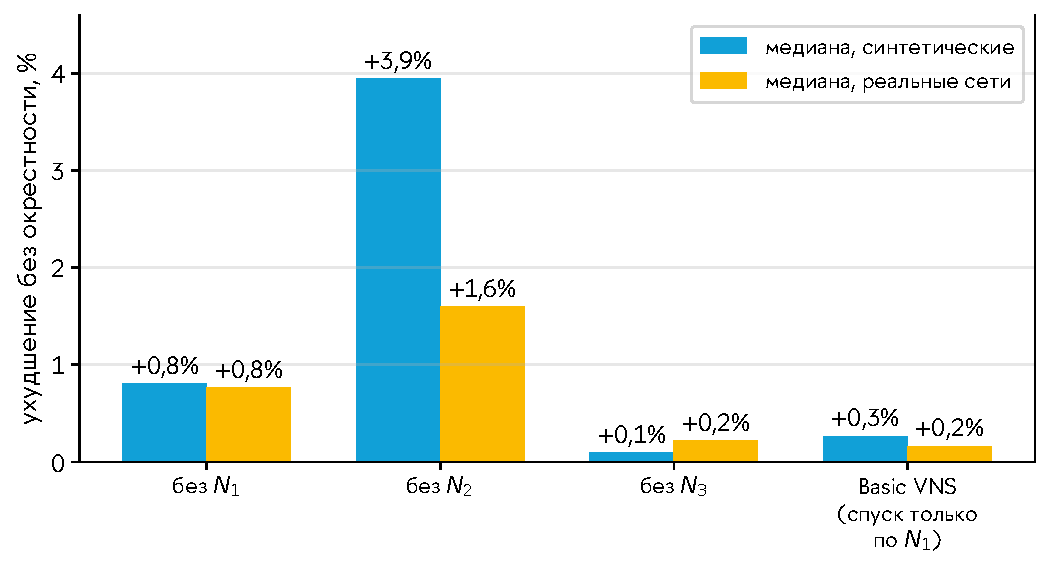
\includegraphics[width=\linewidth]{figs/ablation.pdf}
\source{выключаем одну окрестность, тот же бюджет, лучший из 5 запусков; сети 16--100 складов}
\column{0.44\textwidth}
\begin{itemize}\setlength{\itemsep}{4pt}
\item \textcolor{cN2}{\textbf{$N_2$ --- наибольший вклад}}: её отключение увеличивает стоимость на $3{,}9\%$ на синтетике и на $1{,}6\%$ на реальных сетях (медианы), на отдельной сети --- до $23{,}8\%$
\item \textcolor{cN3}{\textbf{$N_3$ --- полезна при заполненных складах}}: пока ёмкости свободны, её вклад близок к нулю; на сети Германии, где склады заполнены, --- $4{,}0\%$
\item преимущество полного спуска по трём окрестностям над Basic VNS растёт с размером сети: 0,2--0,6\% до 28 складов, 1,1--2,0\% от 50
\end{itemize}
\end{columns}
\end{frame}

% ===========================================================================
\section{Итоги и практика}

\begin{frame}{Основные выводы}
\begin{enumerate}\setlength{\itemsep}{7pt}
\item \textbf{MCF с машинами --- это MILP}: ступенчатая цена линеаризуется целыми $y_e$ и ограничением $f_e\le C y_e$, но LP-релаксация при этом слабая
\item \textbf{пути вместо рёбер}: путей экспоненциально много, но в решении используется небольшое их число; такие пути порождаются генерацией столбцов или эвристикой
\item \textbf{матэвристика}: эвристика сужает пространство до сотен перспективных маршрутов, решатель точно решает маленькую задачу на них
\item \textbf{окрестности отражают структуру задачи}: $N_1$ --- цена перегруза, $N_2$ --- целые машины, $N_3$ --- ёмкость складов
\item \textbf{корректное сравнение}: при неизвестном оптимуме следует измерять отклонение от доказанной нижней оценки
\end{enumerate}
\bigskip
\begin{center}
{\large\itshape\color{hseBlue} Эвристика предлагает возможные пути ---\\решатель выбирает наилучшую комбинацию.}
\end{center}
\end{frame}

\begin{frame}{Практика: конкурс по логистической сети}
\begin{columns}[T]
\column{0.58\textwidth}
\begin{itemize}\setlength{\itemsep}{4pt}
\item условие: модель с ёмкостями складов на приём $U^-_v$ и отправку $U^+_v$ --- \texttt{2026/optimal-logistic-network-contest/MCF\_ext.md}
\item данные: \texttt{reqs.csv} (заявки), \texttt{distance\_matrix.csv} (цены рейсов), \texttt{offices.csv} (перегруз и ёмкости); сети на 10, 20, 50 и 140 узлов
\item решение --- \texttt{paths.csv}: для каждой заявки пути и объёмы
\item проверка и подсчёт стоимости: \texttt{validator\_ext.py}; базовые решения --- в \texttt{baseline/}
\item таблица результатов --- на платформе Яндекс.Контест
\end{itemize}
\column{0.38\textwidth}
\begin{block}{С чего начать}
\begin{enumerate}
\item вычислить валидатором стоимость решения, в котором все заявки перевозятся напрямую
\item решить MILP на пуле из $k$ кратчайших путей
\item разработать собственную окрестность: какие ещё пути предложить решателю?
\end{enumerate}
\end{block}
\end{columns}
\end{frame}

\begin{frame}{Вопросы для самопроверки}
\begin{enumerate}\setlength{\itemsep}{4pt}
\item Почему в задаче о потоке одного товара при целых $u_e$ и $b_v$ у LP-релаксации всегда есть целое оптимальное решение, а для многопродуктового потока это не так? Приведите пример.
\item Чем отличаются постановки на рёбрах и на путях? Почему они эквивалентны?
\item Как линеаризовать стоимость $c_e\lceil f_e/C\rceil$? Почему решатель сам выберет минимальное $y_e$?
\item Почему LP-релаксация этой модели даёт слабую нижнюю оценку?
\item Как в генерации столбцов задача ценообразования сводится к кратчайшему пути?
\item Что даёт лагранжева релаксация ограничений пропускной способности и почему $L(\lambda)\le\text{OPT}$?
\item Почему в GVNS добавление путей в пул не может ухудшить решение?
\item Как сравнивать эвристики, если оптимум неизвестен?
\end{enumerate}
\end{frame}

\begin{frame}{Литература и материалы}
\small
\begin{enumerate}\setlength{\itemsep}{3pt}
\item Ahuja R.\,K., Magnanti T.\,L., Orlin J.\,B. \emph{Network Flows: Theory, Algorithms, and Applications}. Prentice Hall, 1993.
\item Bertsimas D., Tsitsiklis J.\,N. \emph{Introduction to Linear Optimization}. Athena Scientific, 1997.
\item Desrosiers J., Lübbecke M.\,E. A Primer in Column Generation. In: \emph{Column Generation}. Springer, 2005.
\item Mladenović N., Hansen P. Variable neighborhood search. \emph{Computers \& Operations Research}, 24(11), 1997.
\item Maniezzo V., Stützle T., Voß S. (eds.) \emph{Matheuristics: Hybridizing Metaheuristics and Mathematical Programming}. Springer, 2009.
\item Ковалева В., Пономаренко А. Статья о GVNS: \href{https://arxiv.org/abs/2610.30139}{arXiv:2610.30139}; генератор сетей: \href{https://arxiv.org/abs/2606.20653}{arXiv:2606.20653}.
\item Код и данные: \href{https://github.com/aponom84/Optimal-Logistic-Net}{github.com/aponom84/Optimal-Logistic-Net} (код MIT, данные CC BY 4.0).
\item Решатели: \href{https://highs.dev}{HiGHS}, \href{https://www.scipopt.org}{SCIP}, \href{https://developers.google.com/optimization}{Google OR-Tools}.
\end{enumerate}
\end{frame}

\finalframe{Вопросы?}{%
  \begin{tabular}{@{}p{50mm}p{50mm}@{}}
  \tikz\node[fill=white,inner sep=1mm,text=black]{\hypersetup{urlcolor=black}\qrcode[height=15mm]{https://github.com/aponom84/Optimal-Logistic-Net}}; &
  \tikz\node[fill=white,inner sep=1mm,text=black]{\hypersetup{urlcolor=black}\qrcode[height=15mm]{https://arxiv.org/abs/2610.30139}};\\[2pt]
  код и данные проекта & статья на arXiv
  \end{tabular}}

\end{document}
